\documentclass[
	% -- opções da classe memoir --
	12pt,				% tamanho da fonte
	openright,			% capítulos começam em pág ímpar (insere página vazia caso preciso)
	oneside,			% para impressão em verso e anverso. Oposto a oneside
	a4paper,			% tamanho do papel.
	% -- opções da classe abntex2 --
	%chapter=TITLE,		% títulos de capítulos convertidos em letras maiúsculas
	%section=TITLE,		% títulos de seções convertidos em letras maiúsculas
	%subsection=TITLE,	% títulos de subseções convertidos em letras maiúsculas
	%subsubsection=TITLE,% títulos de subsubseções convertidos em letras maiúsculas
	% -- opções do pacote babel --
	english,			% idioma adicional para hifenização
	french,				% idioma adicional para hifenização
	spanish,			% idioma adicional para hifenização
	brazil				% o último idioma é o principal do documento
	]{abntex2}

% ---
% Pacotes básicos
% ---
\usepackage{lmodern}			% Usa a fonte Latin Modern
\usepackage[T1]{fontenc}		    % Selecao de codigos de fonte.
\usepackage[utf8]{inputenc}		% Codificacao do documento (conversão automática dos acentos)
\usepackage{lastpage}			% Usado pela Ficha catalográfica
\usepackage{indentfirst}		    % Indenta o primeiro parágrafo de cada seção.
\usepackage{color}				% Controle das cores
\usepackage{graphicx}			% Inclusão de gráficos
\usepackage{microtype} 			% Para melhorias de justificação
\usepackage{afterpage}
\usepackage{amsmath}            % Pacote para fórmulas matemáticas
\usepackage{amssymb,url}
\usepackage{xcolor,tikz,bm,colortbl}
\usepackage[br]{nicealgo}       % Pacote para criação de algoritmos
\usepackage{customizacoes}

% ---

% ---
% Pacotes adicionais, usados apenas no âmbito do Modelo Canônico do abnteX2
% ---
\usepackage{lipsum}				% Para geração de dummy text
% ---

% ---
% Pacotes de citações
% ---
\usepackage[brazilian,hyperpageref]{backref}	 % Paginas com as citações na bibl
\usepackage[alf]{abntex2cite}	% Citações padrão ABNT
% ---
% CONFIGURAÇÕES DE PACOTES
% ---

% ---
% Configurações do pacote backref
\renewcommand{\familydefault}{\sfdefault}
% Usado sem a opção hyperpageref de backref
\renewcommand{\backrefpagesname}{Citado na(s) página(s):~}
% Texto padrão antes do número das páginas
\renewcommand{\backref}{}
% Define os textos da citação
\renewcommand*{\backrefalt}[4]{
	\ifcase #1 %
		Nenhuma citação no texto.%
	\or
		Citado na página #2.%
	\else
		Citado #1 vezes nas páginas #2.%
	\fi}%
% ---

% ---
% Informações de dados para CAPA e FOLHA DE ROSTO
% ---
\titulo{Título do Texto}
\autor{BEATRIZ DANIEL MONTANHAUR}
\local{Bauru}
\data{2015}
\orientador{Prof. Dr. Seu Orientador}
\instituicao{%
  Universidade Estadual Paulista ``Júlio de Mesquita Filho''
  \par
  Faculdade de Artes, Arquitetura e Comunicação
  \par
  Rádio e TV}
\tipotrabalho{Trabalho de Conclusão de Curso}
% O preambulo deve conter o tipo do trabalho, o objetivo,
% o nome da instituição e a área de concentração
\preambulo{Trabalho de Conclusão de Curso do Curso de Rádio e TV da Universidade Estadual Paulista ``Júlio de Mesquita Filho'', Faculdade de Artes, Arquitetura e Comunicação, Campus Bauru.}
% ---


% ---
% Configurações de aparência do PDF final

% alterando o aspecto da cor azul
\definecolor{blue}{RGB}{41,5,195}

% informações do PDF
\makeatletter
\hypersetup{
     	%pagebackref=true,
		pdftitle={\@title},
		pdfauthor={\@author},
    	pdfsubject={\imprimirpreambulo},
	    pdfcreator={LaTeX with abnTeX2},
		pdfkeywords={abnt}{latex}{abntex}{abntex2}{trabalho acadêmico},
		colorlinks=true,       		% false: boxed links; true: colored links
    	linkcolor=blue,          	% color of internal links
    	citecolor=blue,        		% color of links to bibliography
    	filecolor=magenta,      		% color of file links
		urlcolor=blue,
		bookmarksdepth=4
}
\makeatother
% ---

% ---
% Espaçamentos entre linhas e parágrafos
% ---

% O tamanho do parágrafo é dado por:
\setlength{\parindent}{1.3cm}

% Controle do espaçamento entre um parágrafo e outro:
\setlength{\parskip}{0.2cm}  % tente também \onelineskip

% ---
% compila o indice
% ---
\makeindex
% ---

% ----
% Início do documento
% ----
\begin{document}

% Seleciona o idioma do documento (conforme pacotes do babel)
%\selectlanguage{english}
\selectlanguage{brazil}

% Retira espaço extra obsoleto entre as frases.
\frenchspacing

% ----------------------------------------------------------
% ELEMENTOS PRÉ-TEXTUAIS
% ----------------------------------------------------------
% \pretextual

% ---
% Capa
% ---
\imprimircapa
% ---

% ---
% Folha de rosto
% (o * indica que haverá a ficha bibliográfica)
% ---
\imprimirfolhaderosto*
% ---

% ---
% Inserir a ficha bibliografica
% ---

% Isto é um exemplo de Ficha Catalográfica, ou ``Dados internacionais de
% catalogação-na-publicação''. Você pode utilizar este modelo como referência.
% Porém, provavelmente a biblioteca da sua universidade lhe fornecerá um PDF
% com a ficha catalográfica definitiva após a defesa do trabalho. Quando estiver
% com o documento, salve-o como PDF no diretório do seu projeto e substitua todo
% o conteúdo de implementação deste arquivo pelo comando abaixo:
%
% \begin{fichacatalografica}
%     \includepdf{fig_ficha_catalografica.pdf}
% \end{fichacatalografica}

\begin{fichacatalografica}
	\sffamily
	\vspace*{\fill}					% Posição vertical
	\begin{center}					% Minipage Centralizado
	\fbox{\begin{minipage}[c][8cm]{15.5cm}		% Largura
	\small
	\imprimirautor
	%Sobrenome, Nome do autor

	\hspace{0.5cm} \imprimirtitulo  / \imprimirautor. --
	\imprimirlocal, \imprimirdata-

	\hspace{0.5cm} \pageref{LastPage} p. : il. (algumas color.) ; 30 cm.\\

	\hspace{0.5cm} \imprimirorientadorRotulo~\imprimirorientador\\

	\hspace{0.5cm}
	\parbox[t]{\textwidth}{\imprimirtipotrabalho~--~\imprimirinstituicao,
	\imprimirdata.}\\

	\hspace{0.5cm}
		1. Tags
		2. Para
		3. A
		4. Ficha
		5. Catalográfica
	\end{minipage}}
	\end{center}
\end{fichacatalografica}
% ---

% ---
% Inserir folha de aprovação
% ---

% Isto é um exemplo de Folha de aprovação, elemento obrigatório da NBR
% 14724/2011 (seção 4.2.1.3). Você pode utilizar este modelo até a aprovação
% do trabalho. Após isso, substitua todo o conteúdo deste arquivo por uma
% imagem da página assinada pela banca com o comando abaixo:
%
% \includepdf{folhadeaprovacao_final.pdf}
%
\begin{folhadeaprovacao}

  \begin{center}
    {\ABNTEXchapterfont\large\imprimirautor}

    \vspace*{\fill}\vspace*{\fill}
    \begin{center}
      \ABNTEXchapterfont\bfseries\Large\imprimirtitulo
    \end{center}
    \vspace*{\fill}

    \hspace{.45\textwidth}
    \begin{minipage}{.5\textwidth}
        \imprimirpreambulo
    \end{minipage}%
    \vspace*{\fill}
   \end{center}

   \center Banca Examinadora

   \assinatura{\textbf{\imprimirorientador} \\ Orientador}
   \assinatura{\textbf{Professor} \\ Convidado 1}
   \assinatura{\textbf{Professor} \\ Convidado 2}
   %\assinatura{\textbf{Professor} \\ Convidado 3}
   %\assinatura{\textbf{Professor} \\ Convidado 4}

   \begin{center}
    \vspace*{0.5cm}
    \par
    {Bauru, \_\_\_\_\_ de \_\_\_\_\_\_\_\_\_\_\_ de \_\_\_\_.}
    \vspace*{1cm}
  \end{center}

\end{folhadeaprovacao}
% ---

% ---
% Dedicatória
% ---
\begin{dedicatoria}
   \vspace*{\fill}
   \centering
   \noindent
   \textit{Espaço destinado à dedicátoria do texto.} \vspace*{\fill}
\end{dedicatoria}
% ---

% ---
% Agradecimentos
% ---
\begin{agradecimentos}
Espaço destinado aos agradecimentos.
\end{agradecimentos}
% ---

% ---
% Epígrafe
% ---
\begin{epigrafe}
    \vspace*{\fill}
	\begin{flushright}
		\textit{Espaço destinado à epígrafe.}
	\end{flushright}
\end{epigrafe}
% ---

% ---
% RESUMOS
% ---

% resumo em português
\setlength{\absparsep}{18pt} % ajusta o espaçamento dos parágrafos do resumo
\begin{resumo}

Espaço destinado à escrita do resumo.

\textbf{Palavras-chave:} Palavras-chave de seu resumo.
\end{resumo}

% resumo em inglês
\begin{resumo}[Abstract]
 \begin{otherlanguage*}{english}

Abstract area.

\textbf{Keywords:} Abstract keywords.

 \end{otherlanguage*}
\end{resumo}
% ---

% ---
% inserir lista de ilustrações
% ---
\pdfbookmark[0]{\listfigurename}{lof}
\listoffigures*
\cleardoublepage
% ---

% ---
% inserir lista de tabelas
% ---
\pdfbookmark[0]{\listtablename}{lot}
\listoftables*
\cleardoublepage
% ---

% ---
% inserir lista de abreviaturas e siglas
% ---
% ---

% ---
% inserir o sumario
% ---
\pdfbookmark[0]{\contentsname}{toc}
\tableofcontents*
\cleardoublepage
% ---



% ----------------------------------------------------------
% ELEMENTOS TEXTUAIS
% ----------------------------------------------------------
\pagestyle{simple}

% ----------------------------------------------------------
% Introdução (exemplo de capítulo sem numeração, mas presente no Sumário)
% ----------------------------------------------------------

\chapter{Introdução}
\label{c.introducao}

Para iniciar a produção em .tex é necessário instalar os pacotes básicos da linguagem e seus compiladores. O MiKTeX é um pacote básico para o Windows (miktex.org/download) e o MacTeX um pacote básico para o Mac (tug.org/mactex) que contém o mínimo necessário de TeX/LaTeX para rodar. Ele já vem com os compiladores nativos da linguagem e uma IDE (TeXworks, para edição do texto) que possui o compilador integrado.

Normalmente é utilizado o modo pdfLaTeX + MakeIndex + BibTeX para compilar um arquivo .tex. Existem outros formatos de compiladores, mas essa opção é capaz de gerar um .pdf automático após a compilação e ainda por cima adicionar as funcionalidades do BibTeX (recursos para criação e montagem automática de fontes bibliográficas).

Além disso, também é necessária a instalação do pacote abnTeX2. Esse tutorial https://github.com/abntex/abntex2/wiki/Instalacao provém o passo a passo de como instalar cada componente do TeX, em qualquer sistema operacional (Linux, Mac OS e Windows). Caso esteja utilizando o MiKTeX, ele é capaz de efetuar o download do pacote automaticamente, apenas instale-o, abra o projeto.tex e compile-o, ele irá requisitar a autorização para baixar automaticamente os pacotes que faltam para efetuar a compilação.

Com tudo em mãos e o compilador funcionando, é hora de abrir o modelo (projeto.tex) e começar a escrever o texto. É possível perceber no código a estrutura do arquivo e os campos possíveis de edição. Ao escrever o texto, ele é escrito normalmente, sendo que existem diversos comandos para estilizá-lo, criar tabelas, figuras, dentre outros. A seguir abordaremos os principais comandos e funções que podem ser utilizadas em um projeto básico de TCC. Para outras funções e pacotes, procure no Google, a comunidade é ativa e provavelmente já deve ter feito o que é de sua necessidade.

O arquivo projeto.tex contém os pacotes e comandos básicos que definem a estrutura desse texto já no formato requisitado pela ABNT. Dentro dele é possível ver que estamos importando outros dois arquivos .tex (introducao e conclusao), ou seja, esses arquivos estão sendo basicamente concatenados com o comando ``input''. A divisão não é necessária, mas pode ser que auxilie na escrita do texto  ao deixar as coisas mais separadas e organizadas, não sendo um único arquivo cheio de linhas e linhas de código. 

\section{Modificadores de Texto}
\label{s.modificador}

Os modificadores de texto mais simples utilizados são o negrito (``textbf'') \textbf{texto em negrito} e o itálico (``emph'') \emph{texto em itálico}.

\section{Seções}
\label{s.citacoes}

Seções podem ser criadas a partir do comando ``section'' e hierarquizadas abaixo do capítulo principal. É possível referenciá-las, por exemplo, Seção~\ref{s.citacoes} corresponde a seção atual em que estamos. Já se quisermos referenciar alguma outra coisa, é só utilizarmos o comando ``ref'' presente no código desse texto, por exemplo, Capítulo~\ref{c.introducao}.

\subsection{Subseções}
\label{ss.subsecao}

Subseções também podem ser criadas com o comando ``subsection'' e referenciadas~\ref{ss.subsecao}.

\subsubsection{Sub-subseções}
\label{sss.subsubsecao}

Também há mais um nível que pode ser criado com o comando ``subsubsection''.

\section{Alíneas}
\label{s.alineas}

\begin{alineas}

\item As alineas devem ser criadas desse modo, com o comando begin\{alineas\}. Isso é necessário para que estejam no formato definido pelo pacote abnTeX2 e, consequentemente, no formato definido pela ABNT.

\item Cada item da alínea pode ser invocado com um comando item.

\item O fim de cada alínea é determinado por end\{alineas\}.

\end{alineas}

\section{Tabelas}
\label{s.tabelas}

As tabelas também podem ser referenciadas como se fossem seções ou figuras, por exemplo, esta é a Tabela~\ref{t.transacao_mercado}.

\begin{table}[h]
\centering
\begin{tabular}{c|c}
\hline
\textbf{\small TID} & \textbf{\small Conjunto de Itens}\\\hline \hline
{\small 1} & {\small \{Pão, Leite\}}\\\hline
{\small 2} & {\small \{Pão, Fralda, Cerveja, Ovos\}}\\\hline
{\small 3} & {\small \{Leite, Fralda, Cerveja, Coca-Cola\}}\\\hline
{\small 4} & {\small \{Pão, Leite, Fralda, Cerveja\}}\\\hline
{\small 5} & {\small \{Pão, Leite, Fralda, Coca-Cola\}}\\\hline
\end{tabular}
\caption{Exemplo de transações de mercado.}
\label{t.transacao_mercado}
\end{table}

Quando uma tabela é criada com begin\{table\}, ela é automaticamente adicionada à Lista de Tabelas.

\section{Algoritmos}
\label{s.algoritmos}

O pacote nicealgo incluído nos arquivos desse projeto é responsável por disponibilizar comandos extras, não inerentes ao básico TeX, para a criação de algoritmos. Um exemplo do Algoritmo~\ref{a.algoritmo} é escrito a seguir. Eles também pode ser referenciados como se fossem tabelas ou figuras.

\begin{nicealgo}{a.algoritmo}
\naTITLE{Algoritmo AIS}
\naPREAMBLE
\naINPUT{Conjunto Frequente L = 0 e Grupo de Fronteira F = 0.}
\naBODY
\naBEGIN{\textbf{Enquanto} $F \neq 0$, \textbf{faça}}
\na{\textbf{Seja} conjunto candidato $C = 0$;}
\naBEGIN{\textbf{Para cada} tuplas $t$ da base de dados, \textbf{faça}}
\naBEGIN{\textbf{Para cada} conjuntos de itens $f$ em $F$, \textbf{faça}}
\naBEGIN{\textbf{Se} $t$ contém $f$, \textbf{então}}
\naEND{\textbf{Seja} $C_f =$ conjuntos de itens candidatos extensões de $f$ e contidos em $t$;}
\naBEGIN{\textbf{Para cada} conjunto de itens $c_f$ em $C_f$, \textbf{faça}}
\naBEGIN{\textbf{Se} $c_f \in C$, \textbf{então}}
\naEND{$c_f$.contagem $= c_f$.contagem$ + 1$;}
\naBEGIN{\textbf{Se não}}
\na{$c_f$.contagem $= 0$;}
\naEND{$C = C + c_f$;}
\naEND{}
\naEND{}
\naEND{}
\na{\textbf{Seja} F = 0;}
\naBEGIN{\textbf{Para cada} conjunto de itens $c$ em $C$, \textbf{faça}}
\naBEGIN{\textbf{Se} $contagem(c)/tamanho\_db > minsupport$, \textbf{então}}
\naEND{$L = L + c$;}
\naBEGIN{\textbf{Se} $c$ deve ser usado como a próxima fronteira, \textbf{então}}
\naEND{$F = F + c$;}
\naEND{}
\naEND{}
\end{nicealgo}

\section{Figuras}
\label{s.figuras}

Abaixo podemos identificar a criação e referência da Figura~\ref{f.disposicao_mercado}. Atente-se ao código para perceber um possível redimensionamento com a função scale e o caminho de onde a figura deve ser retirada.

Quando uma figura é criada com begin\{figure\}, ela é automaticamente adicionada à Lista de Ilustrações.

\begin{figure}[h]
\caption{\small Exemplo do ambiente TeXworks.}
\centering
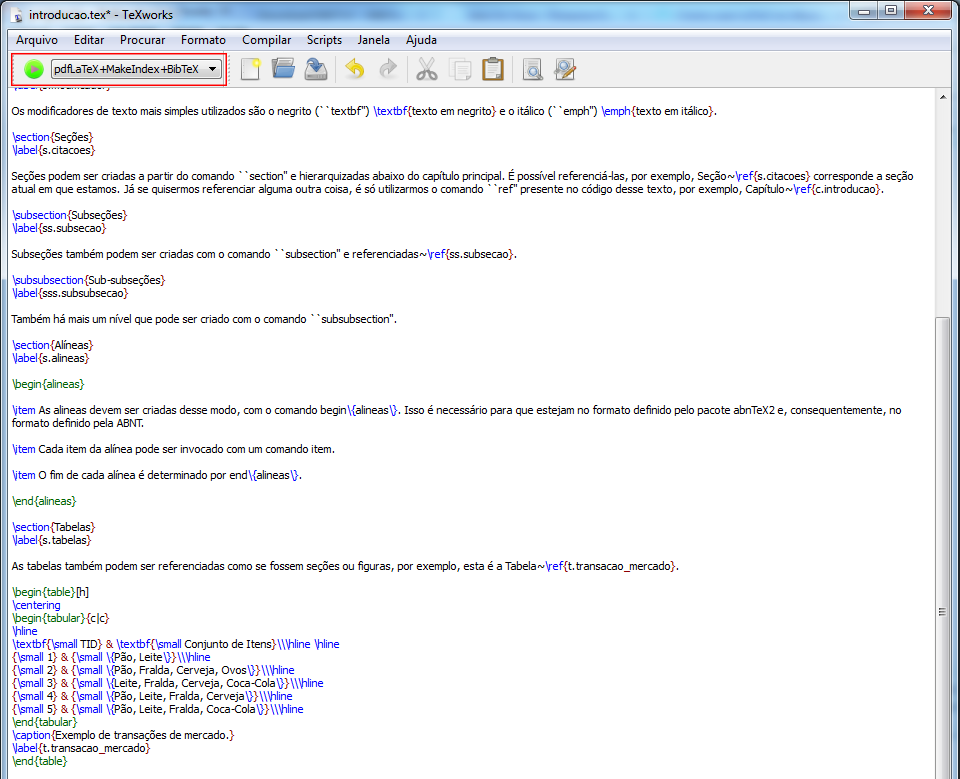
\includegraphics[scale=0.50]{figs/tex_exemplo.png}
\label{f.disposicao_mercado}
\legend{\small Fonte: Elaborada pelo autor.}
\end{figure}

\section{Equações}
\label{s.equacoes}

O TeX também é muito famoso pela forma em que consegue tratar funções e símbolos matemáticos. A partir da utiização de dois cifrões (\$codigo matemático\$) é possível identificar ao compilador que a escrita a seguir são símbolos e códigos originários do pacote matemático do TeX. Aqui estamos demonstrado um exemplo $\phi = 1 + x$ dessa utilização.

Também podemos definir equações utilizando os comandos begin\{equation\} e end\{equation\}. Por exemplo:

\begin{equation}
\label{e.energy_rbm}
E(\textbf{v},\textbf{h})=-\sum_{i=1}^ma_iv_i-\sum_{j=1}^nb_jh_j-\sum_{i=1}^m\sum_{j=1}^nv_ih_jw_{ij},
\end{equation}

\begin{equation}
\label{e.probability_configuration}
P(\textbf{v},\textbf{h})=\frac{e^{-E(\textbf{v},\textbf{h})}}{\displaystyle\sum_{\textbf{v},\textbf{h}}e^{-E(\textbf{v},\textbf{h})}},
\end{equation}

\begin{eqnarray}
\label{eq:par}
\hat{\phi}^j & = & \left\{ \begin{array}{ll} \hat{\phi}^j\pm \varphi_j \varrho  & \mbox{{ com probabilidade PAR}} \\
    \hat{\phi}^j & \mbox{{com probabilidade (1-PAR).}}
\end{array}\right.
\end{eqnarray}

Existem diversos sites no Google que contém códigos de símbolos e funções matemáticas de todos os tipos. Exemplo:\\
\begin{center}
\tiny estudijas.lu.lv/pluginfile.php/14809/mod\_page/content/16/instrukcijas/matematika\_moodle/LaTeX\_Symbols.pdf.
\end{center}

\section{Como citar as referências}
\label{ss.referencias}

Aqui está um exemplo de como podemos referenciar as bibliografias utilizadas no trabalho. Elas são guardadas na forma de metadados (tags) no arquivo .bib a qual é importada no projeto principal (projeto.tex).

E podemos citá-las de acordo com os identificadores atribuídos para cada referência, por exemplo,~\cite{stonebraker93} e~\cite{rocha09}.

Após citar um item de referência bibliográfica com o comando ``cite'', ela será automaticamente padronizada e incluída na página de Referências de seu arquivo. Atualmente os maiores sites portadores de artigos, periódicos, dentre outros (IEEE, Springer, etc) já conseguem exportar a publicação desejado no formato BibTeX, sendo facilmente adicionado ao arquivo .bib de seu trabalho.


\chapter{Conclusão}
\label{c.conclusao}

Os arquivos estão sendo concatenados. Podemos continuar a nossa escrita em outro arquivo .tex desde que ele seja importado no projeto principal, que é sempre o utilizado para efetuar a compilação.

% ---
% Capitulo com exemplos de comandos inseridos de arquivo externo
% ---
% ---

% ----------------------------------------------------------
% ELEMENTOS PÓS-TEXTUAIS
% ----------------------------------------------------------
\postextual
% ----------------------------------------------------------

% ----------------------------------------------------------
% Referências bibliográficas
% ----------------------------------------------------------
\pagestyle{empty}
\bibliography{references} % o arquivo de bibliografia deve ser importando nessa linha sem o .bib

% ----------------------------------------------------------
% Glossário
% ----------------------------------------------------------
%
% Consulte o manual da classe abntex2 para orientações sobre o glossário.
%
%\glossary

%---------------------------------------------------------------------
% INDICE REMISSIVO
%---------------------------------------------------------------------
\phantompart
\printindex
%---------------------------------------------------------------------

\end{document}
